\begin{frame}{$d(K^-, n \pi^{\mp})"\Sigma^{\pm}"$ フィッティング $\d(K^-, n)"X" : 1.35\sim1.44 [GeV/c^2]$}
  \label{page:fitKNpi}
  
  \tminipageFour{
    \begin{figure}
      \centering
      \tiny
      $d(K^-, n)"X" : 1.35 \sim 1.36 [GeV/c^{2}]$
      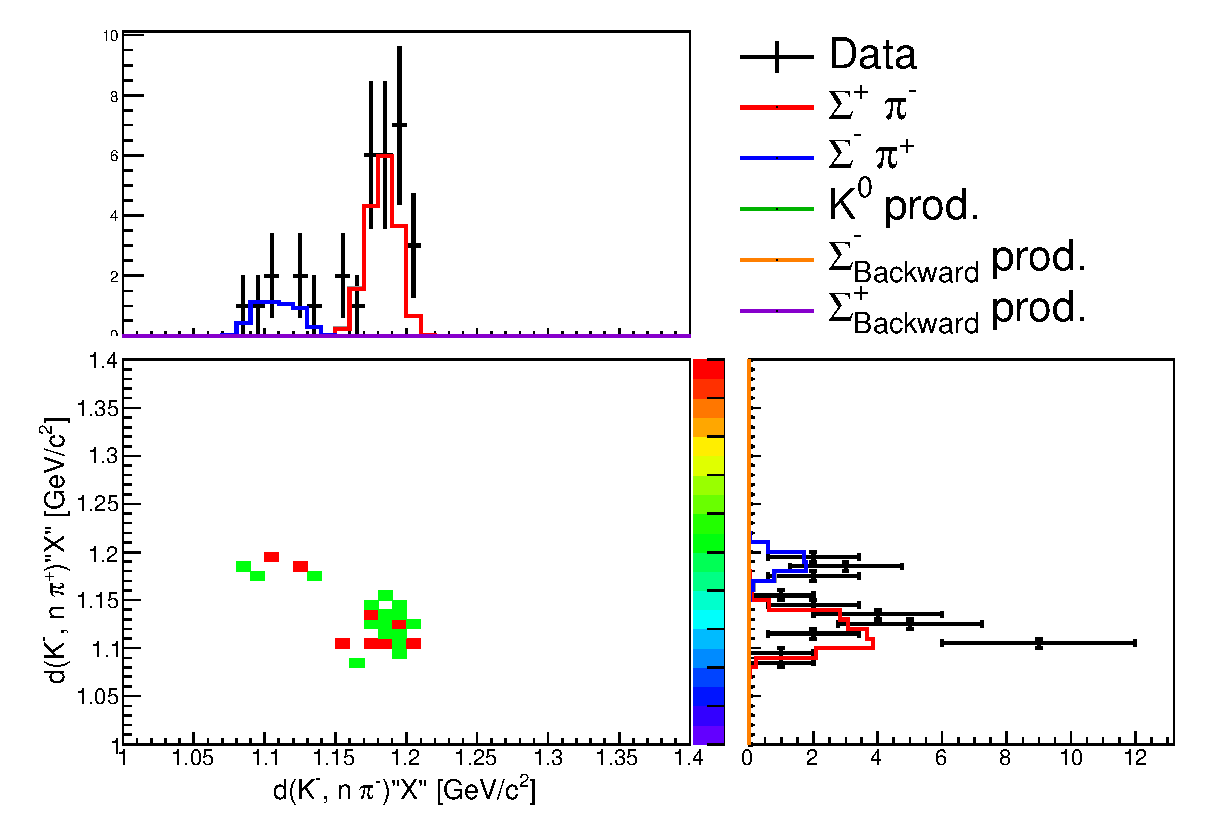
\includegraphics[width=2.5cm]{../pic/Run78/KN_ana_NC170_2sigma/KNpi_MM_1.eps}
    \end{figure}

  }{
    \begin{figure}
      \centering
      \tiny
      $d(K^-, n)"X" : 1.36 \sim 1.37 [GeV/c^{2}]$
      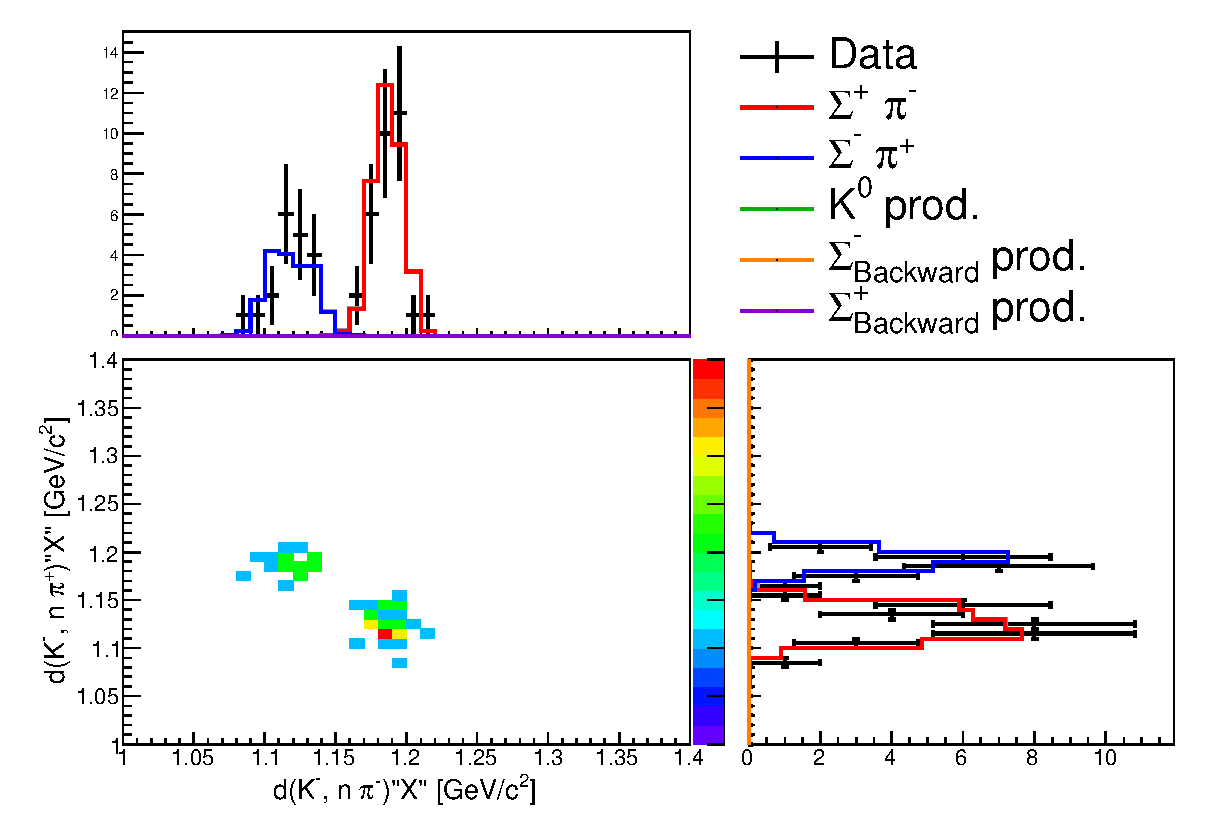
\includegraphics[width=2.5cm]{../pic/Run78/KN_ana_NC170_2sigma/KNpi_MM_2.eps}
    \end{figure}

  }{
    \begin{figure}
      \centering
      \tiny
      $d(K^-, n)"X" : 1.37 \sim 1.38 [GeV/c^{2}]$    
      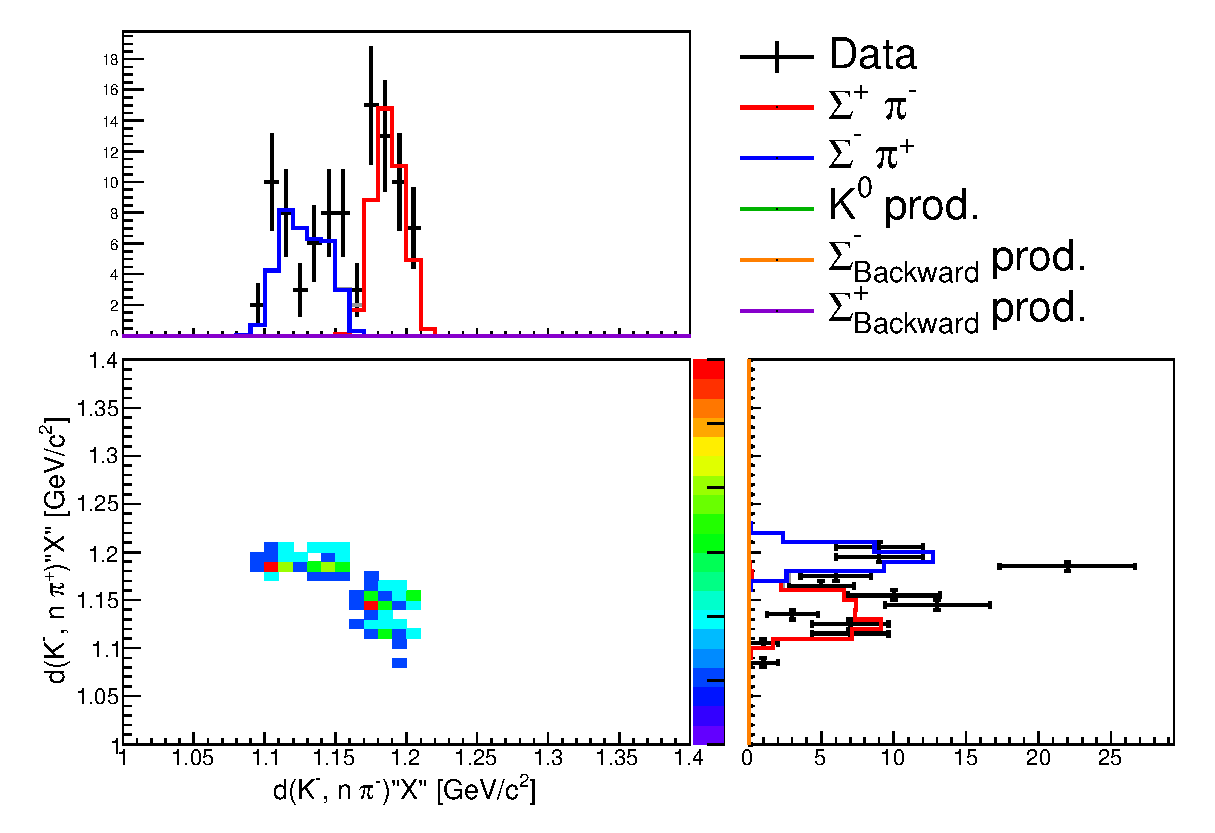
\includegraphics[width=2.5cm]{../pic/Run78/KN_ana_NC170_2sigma/KNpi_MM_3.eps}
    \end{figure}
  }{
    \begin{figure}
      \centering
      \tiny
      $d(K^-, n)"X" : 1.38 \sim 1.39 [GeV/c^{2}]$
      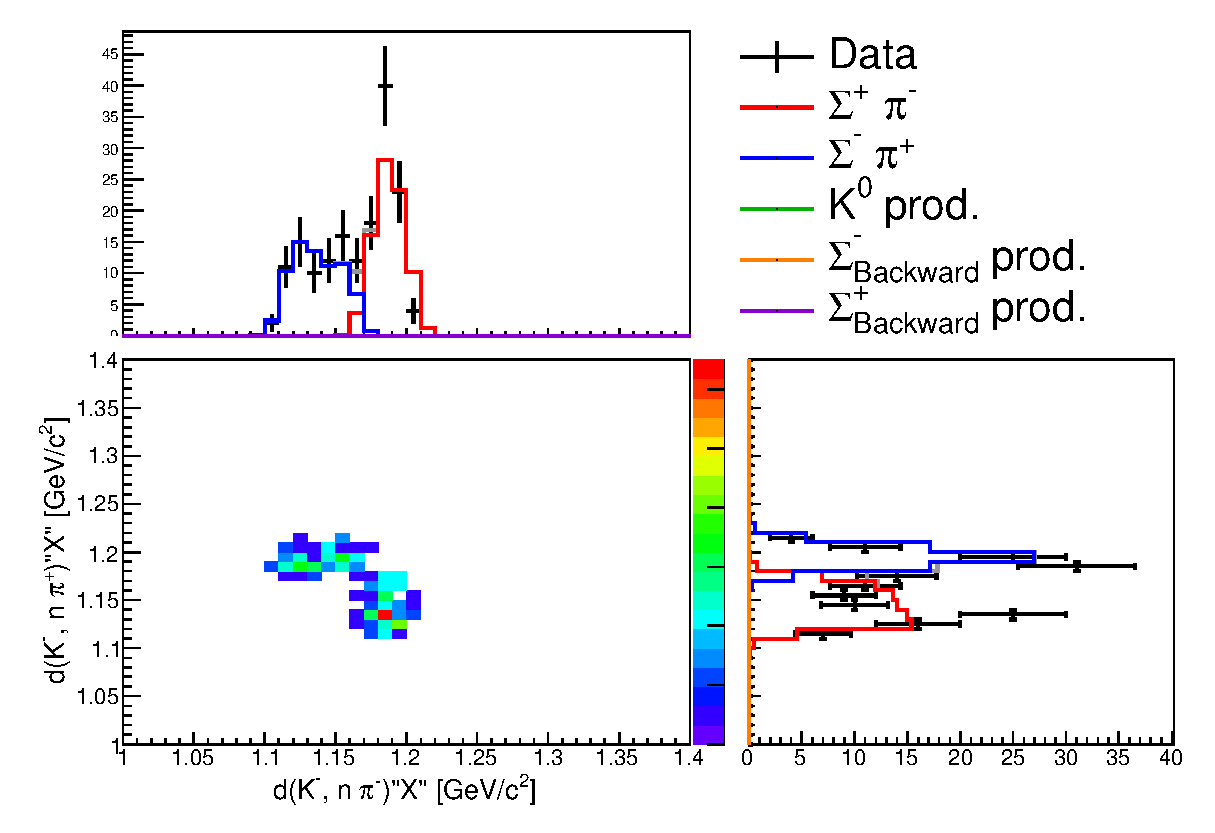
\includegraphics[width=2.5cm]{../pic/Run78/KN_ana_NC170_2sigma/KNpi_MM_4.eps}
    \end{figure}
  }

  \tminipageFour{
    \begin{figure}
      \centering
      \tiny
      $d(K^-, n)"X" : 1.39 \sim 1.40 [GeV/c^{2}]$    
      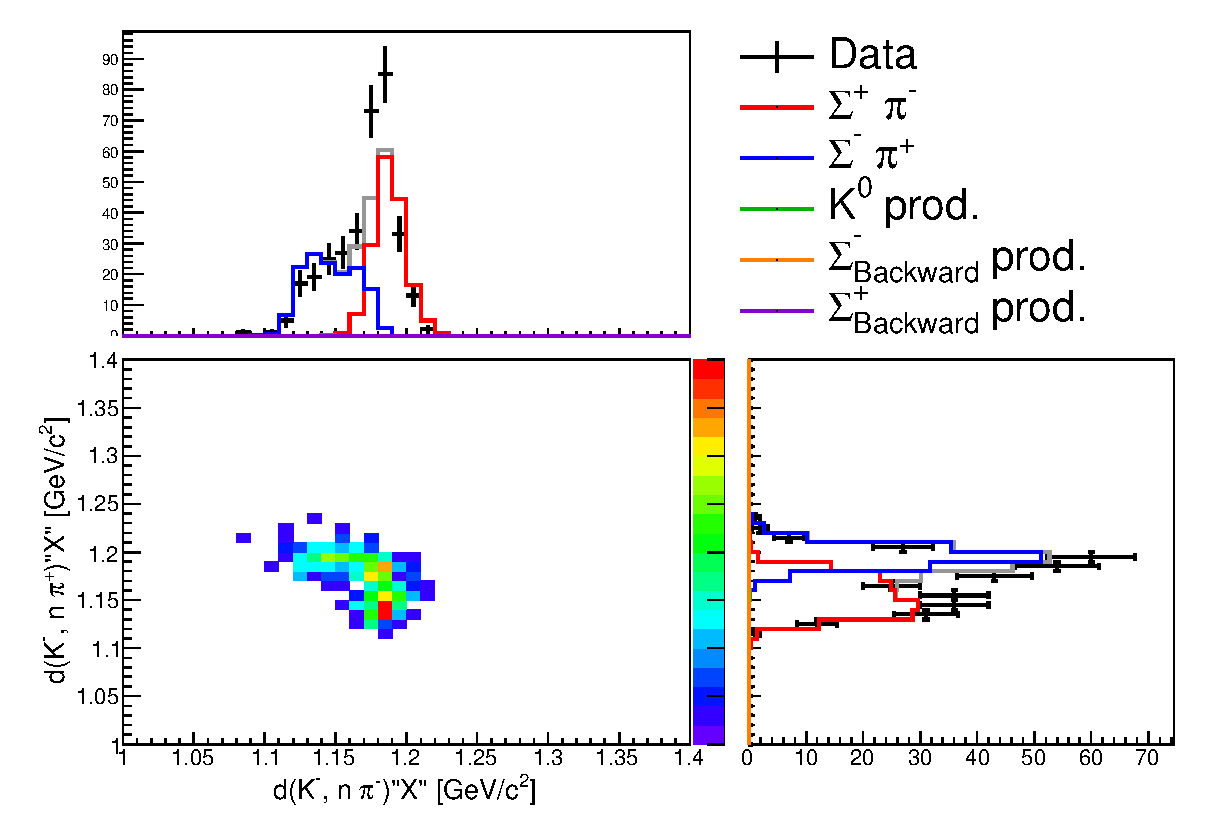
\includegraphics[width=2.5cm]{../pic/Run78/KN_ana_NC170_2sigma/KNpi_MM_5.eps}
    \end{figure}

  }{
    \begin{figure}
      \centering
      \tiny
      $d(K^-, n)"X" : 1.40 \sim 1.41 [GeV/c^{2}]$    
      \includegraphics[width=2.5cm]{../pic/Run78/KN_ana_NC170_2sigma/KNpi_MM_6.eps}
    \end{figure}

  }{
    \begin{figure}
      \centering
      \tiny
      $d(K^-, n)"X" : 1.42 \sim 1.43 [GeV/c^{2}]$
      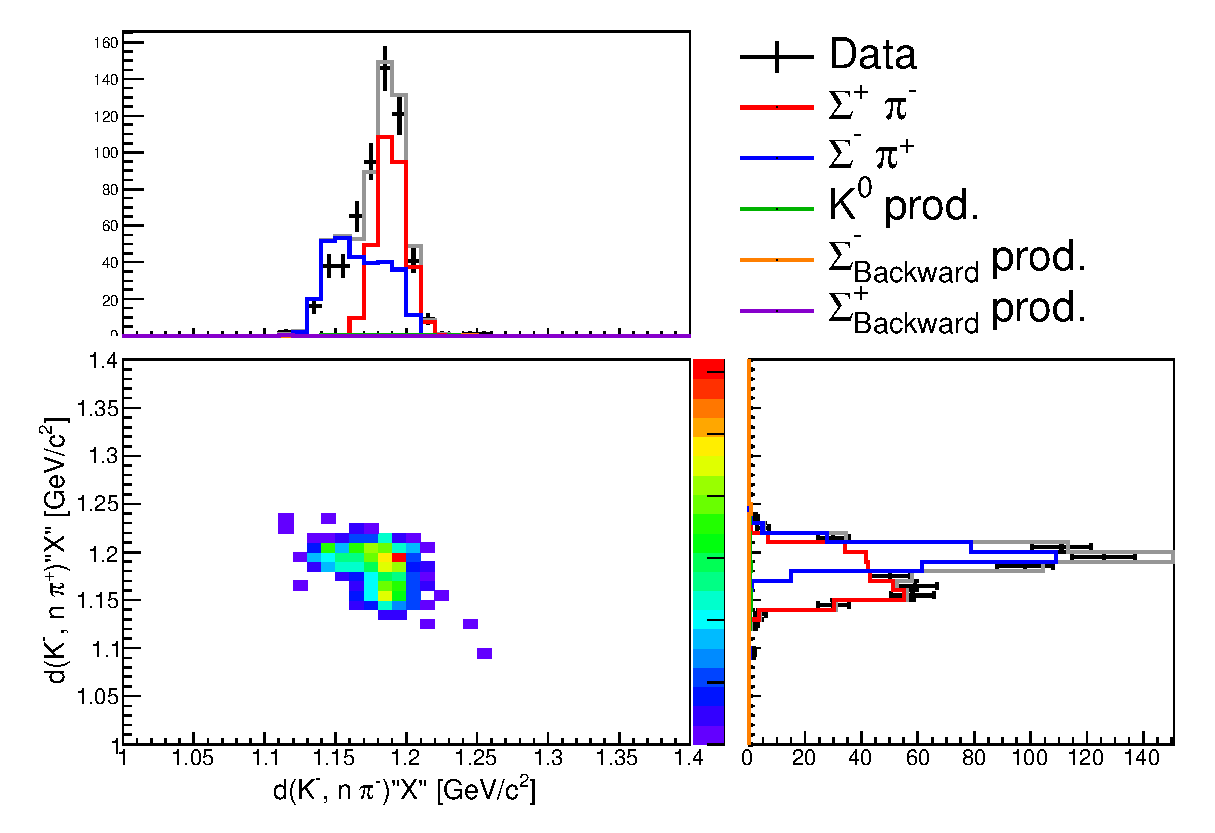
\includegraphics[width=2.5cm]{../pic/Run78/KN_ana_NC170_2sigma/KNpi_MM_7.eps}
    \end{figure}

  }{
    \begin{figure}
      \centering
      \tiny
      $d(K^-, n)"X" : 1.43 \sim 1.44 [GeV/c^{2}]$
      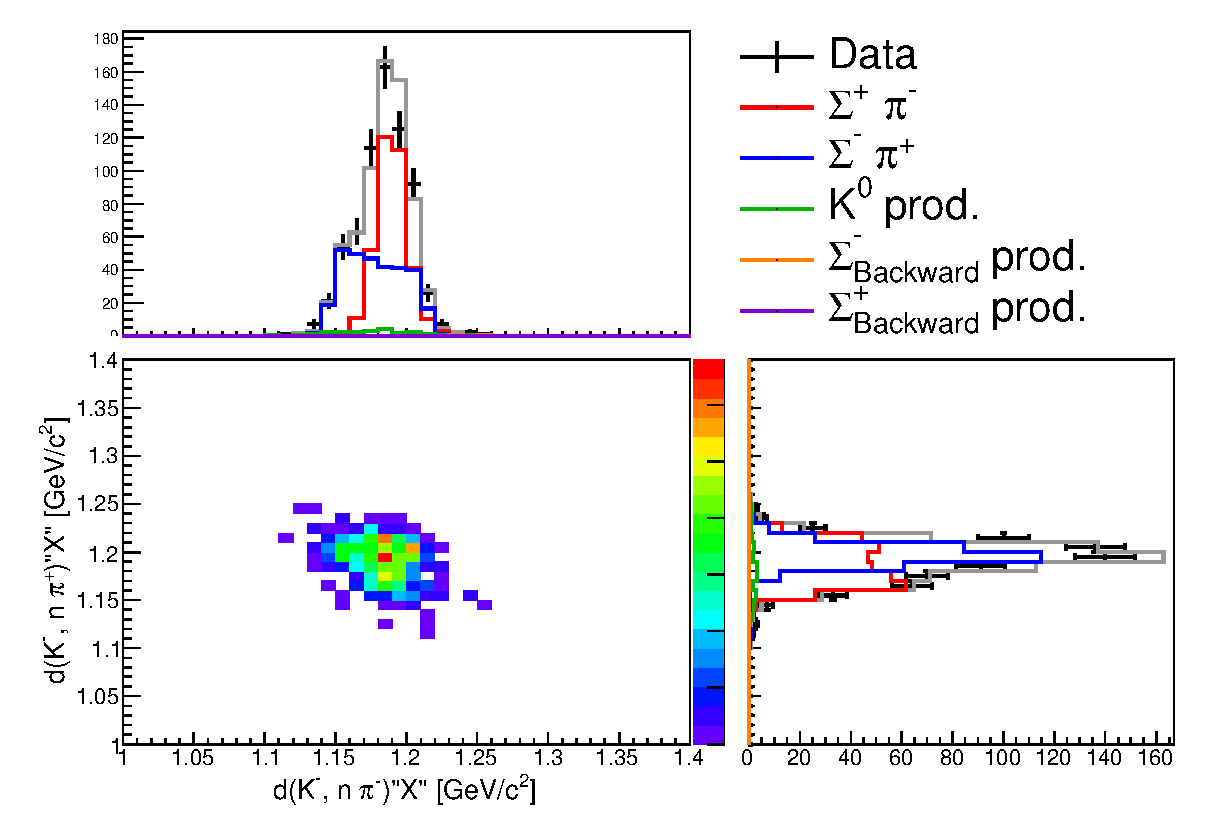
\includegraphics[width=2.5cm]{../pic/Run78/KN_ana_NC170_2sigma/KNpi_MM_8.eps}
    \end{figure}

  }
\end{frame}
